\documentclass[a4paper,11pt]{article}
\input{/home/tof/Documents/Cozy/latex-include/preambule_doc.tex}
\input{/home/tof/Documents/Cozy/latex-include/preambule_commun.tex}
\newcommand{\showprof}{show them}  % comment this line if you don't want to see todo environment
\setlength{\fboxrule}{0.8pt}
\fancyhead[L]{\fbox{\Large{\textbf{Phot 01}}}}
\fancyhead[C]{\textbf{Image numérique}}
\newdate{madate}{10}{09}{2020}
%\fancyhead[R]{\displaydate{madate}} %\today
\fancyhead[R]{Seconde - SNT}
\fancyfoot[L]{\vspace{1mm}Christophe Viroulaud}
\AtEndDocument{\label{lastpage}}
\fancyfoot[C]{\textbf{Page \thepage/\pageref{lastpage}}}
\fancyfoot[R]{\includegraphics[width=2cm,align=t]{/home/tof/Documents/Cozy/latex-include/cc.png}}

\begin{document}
\begin{center}
    \framebox{Comment stocker une image dans un ordinateur?}
\end{center}
\section{Information discrète}
\subsection{Principe de l'argentique}
\begin{center}
    \centering
    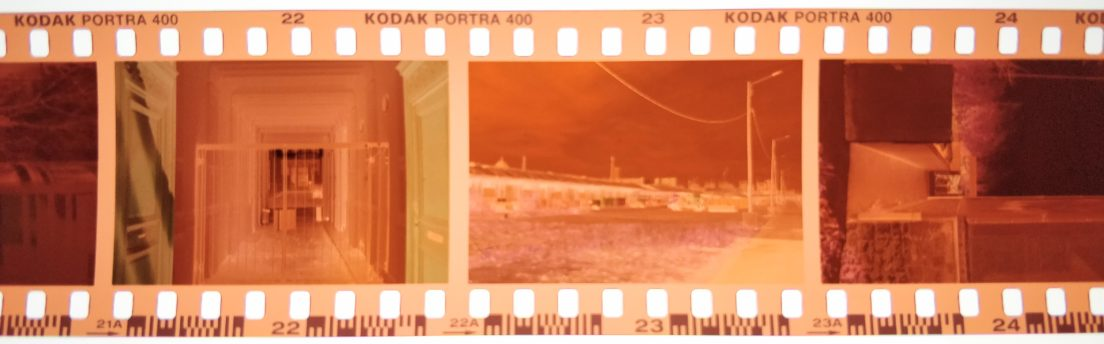
\includegraphics[width=6cm]{ressources/pellicule.jpg}
    \captionof{figure}{Pellicule argentique}
    \label{IMG}
\end{center}
\begin{aretenir}[]
    Dans une photographie argentique, les informations de l'image sont \textbf{continues}.
\end{aretenir}
\subsection{Principe du numérique}
\begin{center}
    \centering
    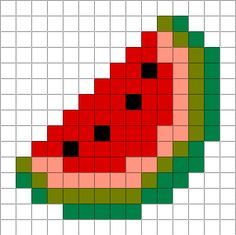
\includegraphics[width=4cm]{ressources/pasteque.jpg}
    \captionof{figure}{ Dans un ordinateur, une image est découpée en petits morceaux.}
    \label{IMG}
\end{center}
\begin{aretenir}[]
    Une image numérique est découpée en \textbf{pixels}. L'information de chaque pixel est une donnée \textbf{discrète}.
\end{aretenir}
\section{Caractéristiques d'une image numérique}
\subsection{Dimensions}
\begin{center}
    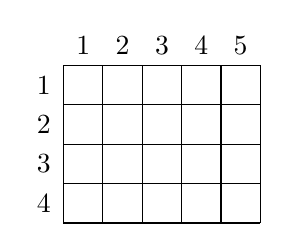
\begin{tikzpicture}[scale=0.5]
        \draw (0,0) grid (5,4);

        \draw (-0.5,3.5) node{1};
        \draw (-0.5,2.5) node{2};
        \draw (-0.5,1.5) node{3};
        \draw (-0.5,0.5) node{4};
        \draw (0.5,4.5) node{1};
        \draw (1.5,4.5) node{2};
        \draw (2.5,4.5) node{3};
        \draw (3.5,4.5) node{4};
        \draw (4.5,4.5) node{5};
    \end{tikzpicture}
    \label{matrice}
\end{center}
\begin{itemize}
    \item La \textbf{définition} d'une image de \emph{m} lignes et \emph{n} colonnes est $m×n$. L'image a une définition de $5×4=20~pixels$.
    \item La \textbf{résolution} est le nombre de pixels par unité de longueur. On utilise couramment l'unité américaine (le \emph{pouce}).
    \item Il existe plusieurs \textbf{formats} d'image: \emph{bitmap (bmp)}, \emph{jpeg} (Joint Photographic Experts Group) ou \emph{png} (Portable Network Graphics).
\end{itemize}
\subsection{Couleurs}
\subsubsection{Synthèse additive}
\begin{aretenir}[]
    À partir de trois sources lumineuses primaires (\emph{Rouge, Vert, Bleu - RVB ou RGB en anglais}) il est possible d'obtenir une grande variété d'autres couleurs.
\end{aretenir}
\begin{itemize}
    \item Dans une image numérique chaque couleur peut varier de 0 à 255 soit 256 valeurs.
          \begin{aretenir}[]
              Avec ce système on peut créer $256×256×256=16777216$, soit plus de 16 millions de couleurs.
          \end{aretenir}
    \item Les couleurs:
          \begin{itemize}
              \item rouge: \#FF0000
              \item vert: \#00FF00
              \item bleu: \#0000FF
          \end{itemize}
\end{itemize}
\begin{aretenir}[]
    \begin{itemize}
        \item Une image numérique peut contenir plusieurs millions de pixels.
        \item Chaque pixel est une couleur parmi plus de 16 millions possibles.
    \end{itemize}
    \end{aretenir}
    \subsubsection{Synthèse soustractive}
    Une imprimante à jet d'encre utilise quatre encres: \emph{Cyan, Magenta, Jaune, Noir}. En appliquant les trois premières couleurs sur une feuille blanche il est possible de créer les autres nuances par \emph{synthèse soustractive}.
\end{document}